\documentclass[a4paper]{article}
\usepackage[utf8]{inputenc}
\usepackage{textcomp}
\usepackage{geometry}
\geometry{ left=2cm, right=2cm, top=2cm, bottom=2cm, bindingoffset=5mm}
\usepackage{graphicx}
\usepackage{xcolor}
\usepackage{hyperref}
\date{}
\author{}
\usepackage{fancyhdr}
\pagestyle{fancy}
\fancyhf{}
\fancyhead[R]{Felix Bühler - 2973140\\ Jan Leusmann - 2893121\\  Jamie Ullerich - 3141241}
\fancyhead[L]{Reinforcement Learning \\ SS 2020}
\renewcommand{\headrulewidth}{0.5pt}
\usepackage{tikz}
\usetikzlibrary{calc}
\usepackage{amsmath}
\usepackage{cleveref}
\usepackage{subcaption}
\usepackage{array}
\usepackage{bbold}
\usepackage{listings}

\title{\textbf{Exercise 8}}

\begin{document}
\maketitle 
\thispagestyle{fancy}

\section*{Task 1 - REINFORCE on the Cart-Pole}

\subsection*{a)}
Action $a_1$: $\pi (a_1 | s, \theta) = \dfrac{e^{h(s, a_1, \theta)}}{e^{h(s, a_1, \theta)} + e^{h(s, a_2, \theta)}}$ \\ \linebreak
Action $a_2$: $\pi (a_2 | s, \theta) = \dfrac{e^{h(s, a_2, \theta)}}{e^{h(s, a_1, \theta)} + e^{h(s, a_2, \theta)}}$ \\ \linebreak
Derivative: 
%$h(s, a, \theta) = \theta^T_a s$
%TODO solution here or from deeplearning: https://eli.thegreenplace.net/2016/the-softmax-function-and-its-derivative/
\begin{align*}
\pi(a|s, \theta) &= \dfrac{e^{h(s, a, \theta)}}{\sum_{b}e^{h(s, b, \theta)}} \\
\log(\pi(a|s, \theta) ) &= \log(e^{h(s, a, \theta)}) - \log(\sum_{b}e^{h(s, b, \theta)}) 
\end{align*}
$\rightarrow$ gradient: 
\begin{align*}
	\nabla_{\theta} \log(\pi(a|s, \theta) ) &= \nabla_{\theta} \log(e^{h(s, a, \theta)}) - \nabla_{\theta} \log(\sum_{b}e^{h(s, b, \theta)}) \\
	&= \nabla_{\theta} (h(s, a, \theta)) - \dfrac{\nabla_{\theta} \sum_{b}e^{h(s,b,\theta)}}{ \sum_{b}e^{h(s,b,\theta)}}\\
	&= \nabla_{\theta} (\theta^T_a s) - \nabla_{\theta} \sum_{b} \theta^T_b s \ \pi(b|s, \theta) \\
	%&= s -\sum_{b} s \pi(a|s, \theta)
\end{align*}
\subsection*{b)}
\begin{align*}
	\nabla_{\theta} \log \pi (A_t | S_t, \theta) &= ... \\
	%TODO (solution found online)
	 &= x(s, a) - \sum_{b}^{}(q_{\pi}(s, a) - b(s)) \nabla(a|s, \theta)
\end{align*}

\subsection*{c)}
\begin{figure}[!ht]
	\centering
	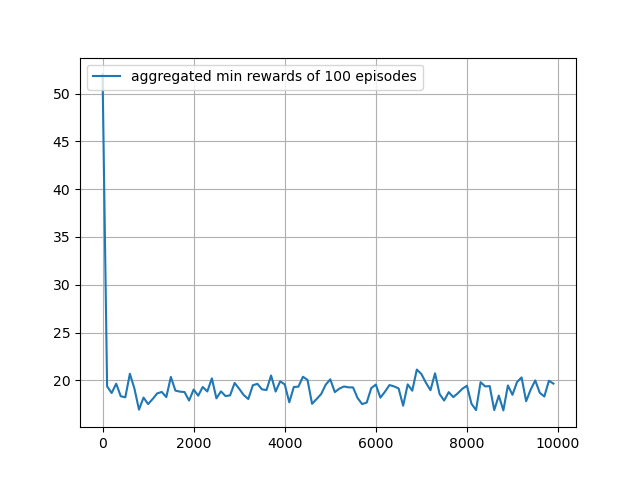
\includegraphics[width=0.7\linewidth]{length}
	\caption{average episode lengths}
	\label{fig:length}
\end{figure}

\subsection*{d)}


\end{document}
